\documentclass[11pt,a4]{article}
\usepackage[cm]{fullpage}
\usepackage{graphicx}
\usepackage{subfigure}
\usepackage{epsfig}
\usepackage{epstopdf}
\begin{document}

\begin{figure}[h]
\centering
    \includegraphics[width=0.49\textwidth]{YY1}
    \includegraphics[width=0.49\textwidth]{SP2}
    \includegraphics[width=0.49\textwidth]{REST}
    \includegraphics[width=0.49\textwidth]{SIX5}
\caption{ROC curve created when applying the methods to data from the cell line H1-hESC. All HMM Models were trained with data from H1-hESC and K562 cell lines.}
\label{fig:roc.H1hesc.1}
\end{figure}

\begin{figure}[h]
\centering
    \includegraphics[width=0.49\textwidth]{BRCA1}
    \includegraphics[width=0.49\textwidth]{TCF12}
    \includegraphics[width=0.49\textwidth]{EGR1}
    \includegraphics[width=0.49\textwidth]{RAD21}
\caption{ROC curve created when applying the methods to data from the cell line H1-hESC. All HMM Models were trained with data from H1-hESC and K562 cell lines.}
\label{fig:roc.H1hesc.2}
\end{figure}

\begin{figure}[h]
\centering
    \includegraphics[width=0.49\textwidth]{ATF3}
    \includegraphics[width=0.49\textwidth]{NRF1}
    \includegraphics[width=0.49\textwidth]{USF2}
    \includegraphics[width=0.49\textwidth]{JUND}
\caption{ROC curve created when applying the methods to data from the cell line H1-hESC. All HMM Models were trained with data from H1-hESC and K562 cell lines.}
\label{fig:roc.H1hesc.3}
\end{figure}

\begin{figure}[h]
\centering
    \includegraphics[width=0.49\textwidth]{ZNF143}
    \includegraphics[width=0.49\textwidth]{BACH1}
    \includegraphics[width=0.49\textwidth]{SP4}
    \includegraphics[width=0.49\textwidth]{MAFK}
\caption{ROC curve created when applying the methods to data from the cell line H1-hESC. All HMM Models were trained with data from H1-hESC and K562 cell lines.}
\label{fig:roc.H1hesc.4}
\end{figure}

\begin{figure}[h]
\centering
    \includegraphics[width=0.49\textwidth]{MYC}
    \includegraphics[width=0.49\textwidth]{SRF}
    \includegraphics[width=0.49\textwidth]{JUN}
    \includegraphics[width=0.49\textwidth]{TBP}
\caption{ROC curve created when applying the methods to data from the cell line H1-hESC. All HMM Models were trained with data from H1-hESC and K562 cell lines.}
\label{fig:roc.H1hesc.5}
\end{figure}

\begin{figure}[h]
\centering
    \includegraphics[width=0.49\textwidth]{P300}
    \includegraphics[width=0.49\textwidth]{FOSL1}
    \includegraphics[width=0.49\textwidth]{USF1}
    \includegraphics[width=0.49\textwidth]{RXRA}
\caption{ROC curve created when applying the methods to data from the cell line H1-hESC. All HMM Models were trained with data from H1-hESC and K562 cell lines.}
\label{fig:roc.H1hesc.6}
\end{figure}

\begin{figure}[h]
\centering
    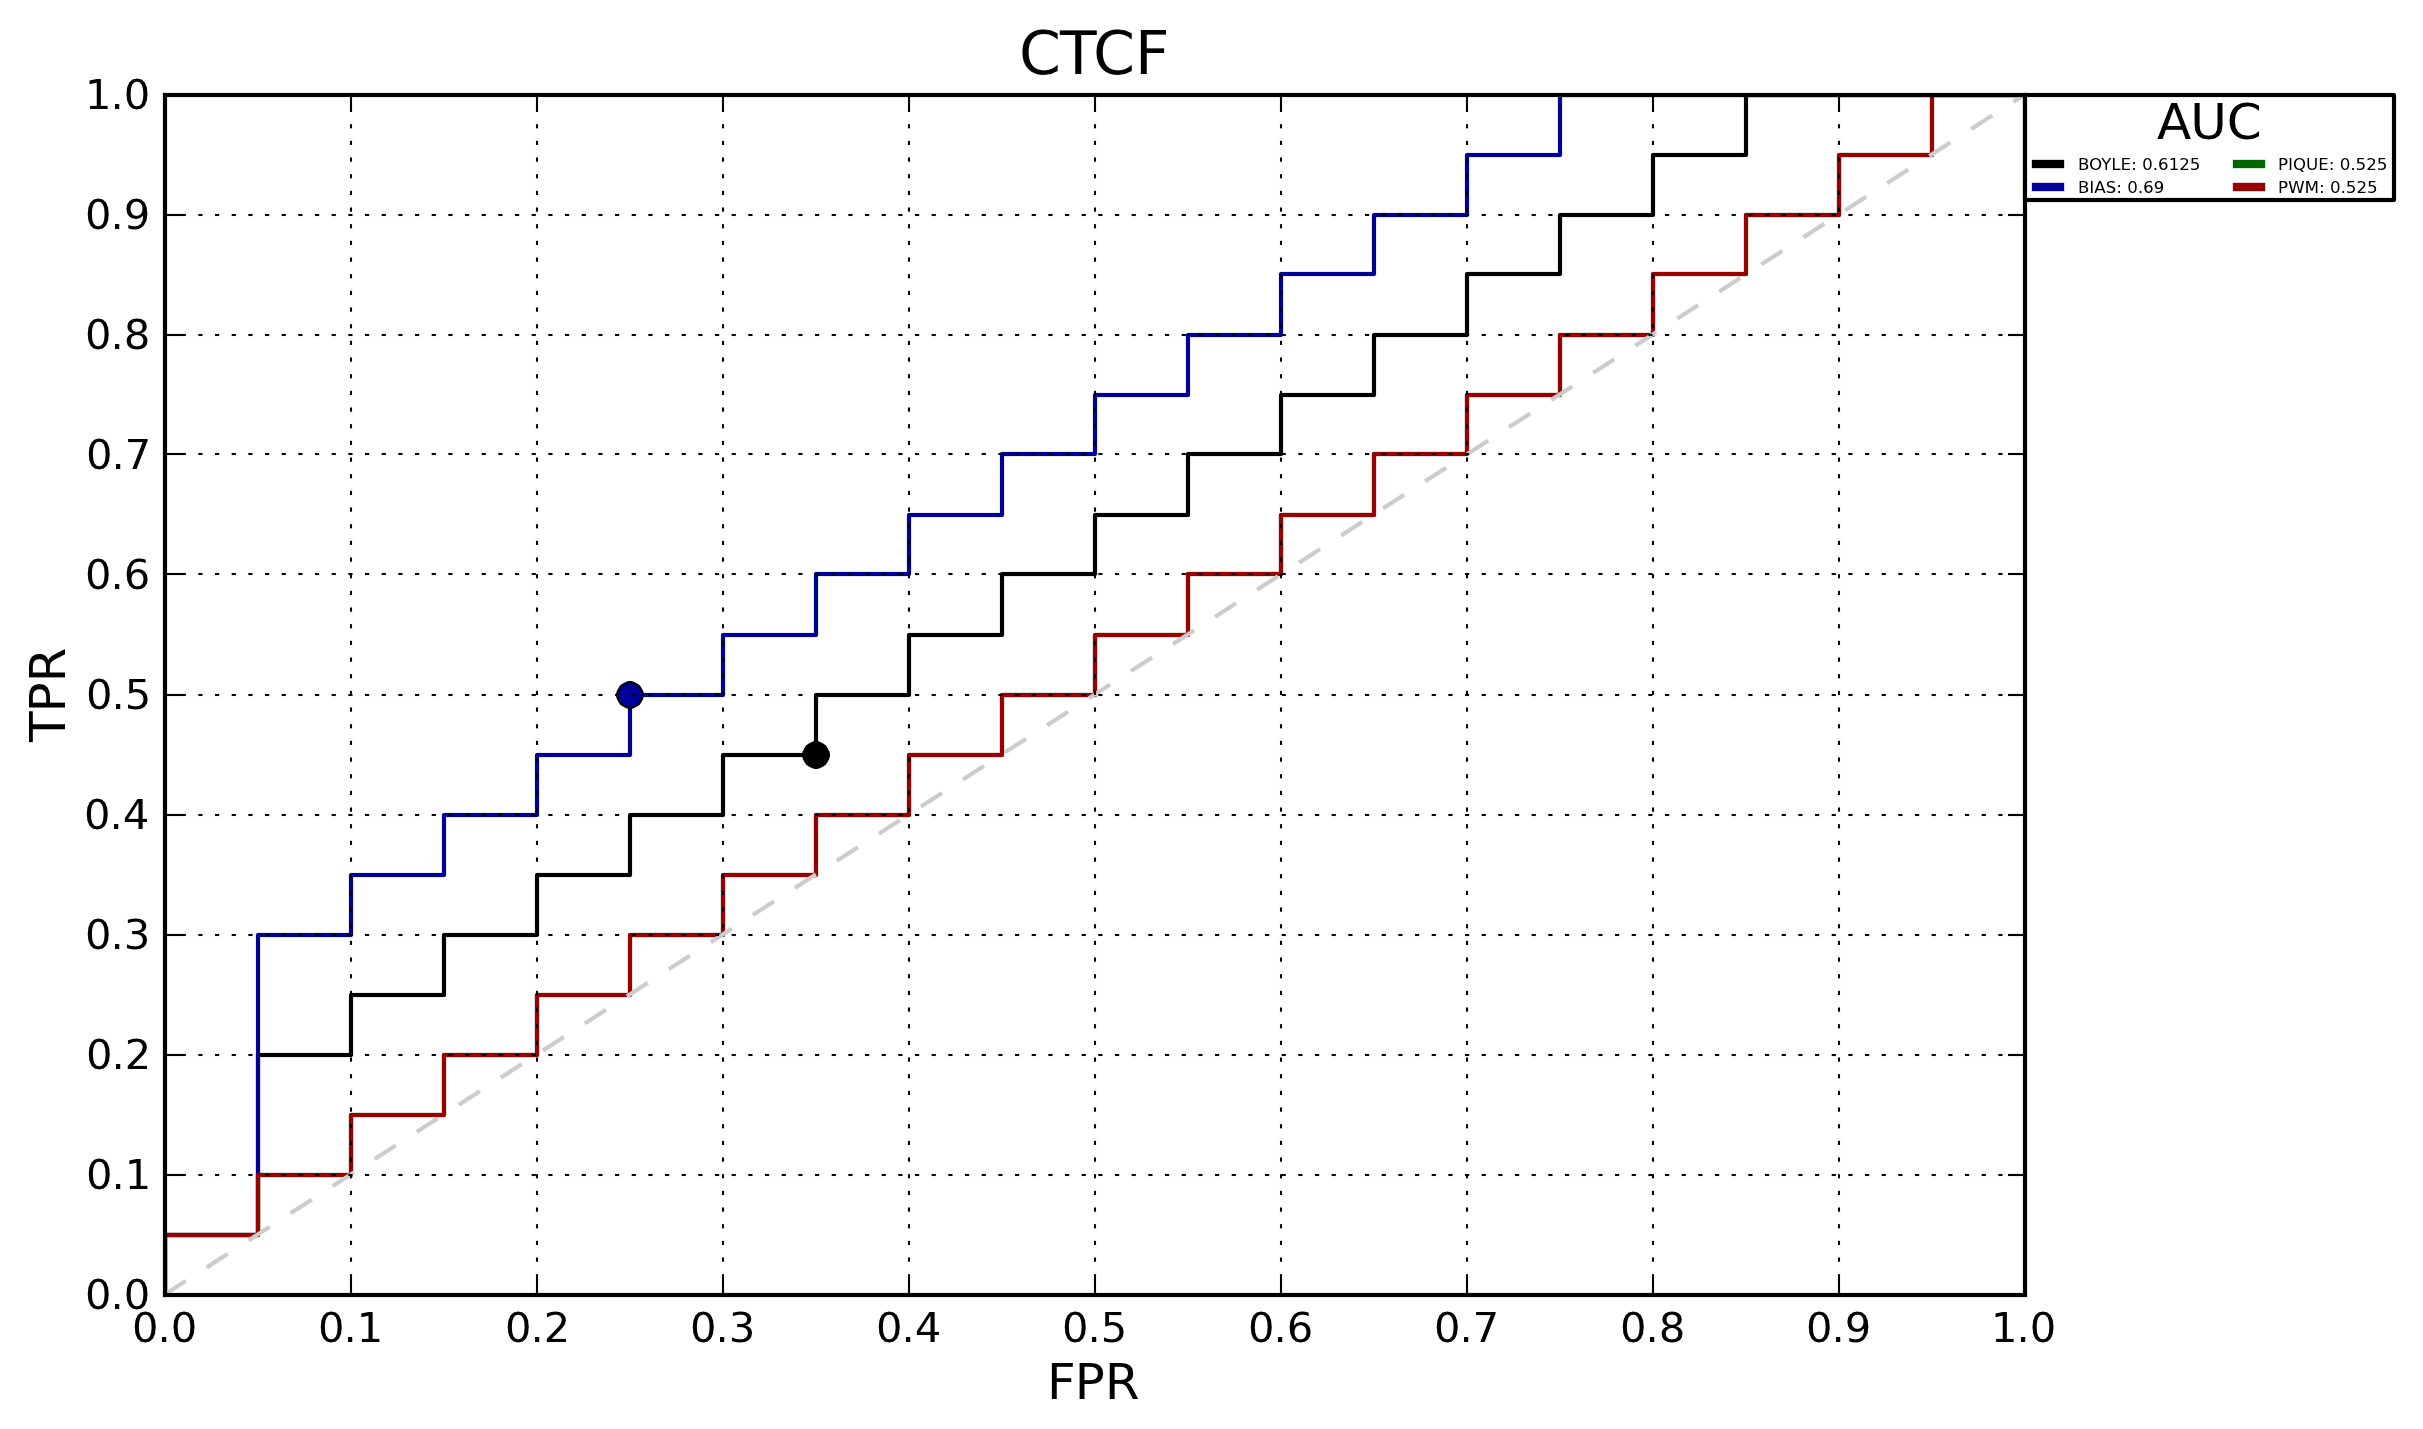
\includegraphics[width=0.49\textwidth]{CTCF}
    \includegraphics[width=0.49\textwidth]{RFX5}
    \includegraphics[width=0.49\textwidth]{POU5F1}
    \includegraphics[width=0.49\textwidth]{MAX}
\caption{ROC curve created when applying the methods to data from the cell line H1-hESC. All HMM Models were trained with data from H1-hESC and K562 cell lines.}
\label{fig:roc.H1hesc.7}
\end{figure}

\begin{figure}[h]
\centering
    \includegraphics[width=0.49\textwidth]{SP1}
    \includegraphics[width=0.49\textwidth]{CEBPB}
    \includegraphics[width=0.49\textwidth]{GABP}
\caption{ROC curve created when applying the methods to data from the cell line H1-hESC. All HMM Models were trained with data from H1-hESC and K562 cell lines.}
\label{fig:roc.H1hesc.8}
\end{figure}

\end{document}